% -*- mode: fundamental -*-

% ****************************************************************

\chapter{Overview of the RISC-V ISA}

\markboth{Ch \arabic{chapter}: RISC-V ISA Overview (DRAFT)}{\copyrightnotice}


\setcounter{page}{1}
% \renewcommand{\thepage}{\arabic{page}}
\renewcommand{\thepage}{\arabic{chapter}-\arabic{page}}

\label{ch_ISA}

% ****************************************************************

\section{Introduction}

This entire chapter can safely be skipped by those already familiar
with RISC-V concepts, or who learn it elsewhere (there are many
alternate resources on the web).  This chapter contains only generic
information about ISAs and the RISC-V ISA in particular.  It can be
read as a general introduction to the RISC-V universe; none of this is
specific to this book.

% ****************************************************************

\section{What is an ISA?}

\index{RISC-V!ISA!Instruction Set Architecture}

The acronym ``ISA'' stands for ``Instruction Set Architecture''.
Figure~\ref{Fig_What_is_an_ISA} illustrates the role of an ISA as an
intermediary between hardware (CPU implementations) and software
(which runs on the CPU hardware).
\begin{figure}[htbp]
  \centerline{\includegraphics[width=6in,angle=0]{Figures/Fig_What_is_an_ISA}}
  \caption{\label{Fig_What_is_an_ISA} What is an ISA?}
\end{figure}

An ISA, \emph{per se}, is neither software nor hardware.  It is merely
a \emph{specification}, a document defining three things:

\begin{itemize}

  \index{RISC-V!ISA!Architectural State}
  \index{RISC-V!ISA!Program Counter, PC}
  \index{RISC-V!ISA!PC, Program Counter}
  \index{RISC-V!ISA!Register File}

  \item \emph{Architectural State}: the registers visible to the
        instructions, such as the program counter (PC) and a register
        file containing, say, 32 registers named x0 through x31.

        Typically (nowadays), the architectural state includes a
        \emph{byte-addressed} memory (a memory where an \emph{address}
        identifies a single byte, and where individual bytes may be
        read and written.

  \index{RISC-V!ISA!Instruction Set}
  \index{RISC-V!ISA!Instruction Set encoding in bits}
  \index{RISC-V!ISA!Assembly Language}

  \item An \emph{Instruction Set}: a collection of instructions.  For
        each instruction, the ISA specifies how it is encoded in bits.
        The ISA may also specify a way of writing an instruction in
        symbolic text, which we call Assembly Language.  Instructions
        are typically grouped in classes, such as Immediate,
        LOAD/STORE, Arithmetic and Logic, Conditional Branches, Jumps,
        System Instructions, and so on.

  \index{RISC-V!ISA!Instruction semantics}

  \item \emph{Semantics}: a description, for each instruction about
        \emph{how} it executes---what architectural state it observes,
        and what architectural state it updates, and how.  For
        example, a Conditional Branch instruction typically observes
        two registers in the register file, compares them, and updates
        the PC depending on the comparison result.

        The overal semantics of a program being executed is just a
        sequential composition of individual instruction semantics.

\end{itemize}

\index{RISC-V!ISA!Formal Specification in Sail}
\index{RISC-V!ISA!Sail Formal Specification language}

The full ISA may be described in ordinary text prose and diagrams, or
in a semi-formal or formal language.  For example, the RISC-V ISA is
described both in text prose and diagrams, and in the formal language
``Sail''.

\index{RISC-V!Micro-architecture}
\index{RISC-V!Micro-architecture!Superscalar}
\index{RISC-V!Micro-architecture!Out-of-order}
\index{RISC-V!Micro-architecture!Pipelining}
\index{RISC-V!Micro-architecture!Speculation}
\index{RISC-V!Micro-architecture!Multi-threaded}
\index{RISC-V!Micro-architecture!Multi-core}

Beneath the ISA level are actual \emph{implementations} of the ISA.
These range from software simulators of the ISA to silicon
implementations.  Silicon implementations typically vary widely in
their \emph{micro-architecture} features, such as pipelining, in-order
or out-of-order, speculation, superscalarity, multi-threading,
multi-core.  The choice of micro-architecture is typically based on a
particular target market, trading-off cost, performance (speed),
energy consumption, capabilities (embedded software to full server OS
with network and storage stacks), silicon technology (FPGA {\vs} ASIC,
ASICs with various silicon feature sizes and techniques), and so on.
Variations in micro-architectures provide product differentiation.

\index{RISC-V!Machine code}

Each implementation runs (interprets) machine code, {\ie} an encoding
of instructions in memory.  The machine codes are typically produced
by compilers, which are themselves machine code programs that
transform source codes into machine codes.  Some machine codes are
themselves software interpreters for so-called interpreted languages
such as Python, Javascript, Java, Scheme, Lisp, and so on.

A crucially important point is that \emph{all the implementations of
an ISA should respect the semantics of the ISA as specified in the ISA
definition}.  They can (and do) play all kinds of micro-architectural
tricks under the covers, but the result of executing any program
should be explainable purely based on the ISA specification.

\index{RISC-V!ISA!Enables software portability}
\index{RISC-V!ISA!Contract between software and hardware implementations}

Thus, and ISA is a \emph{contract} or \emph{API} between software and
hardware implementations.  People writing software, people writing
compilers for software, people writing interpreters for interpreted
languages, {\etc} need only to understand and refer to the ISA
specification to do their job.  They do not need to know about the
specific hardware implementation on which it will eventually run.
This enables \emph{software portability}, {\ie} a machine code program
for an ISA should be able to run, without change, on \emph{any}
implementation of the ISA, including future next-generation
laptops/servers for the ISA.

% ----------------
\vspace{2ex}

NOTE:
\fbox{\small
\begin{minipage}{5in}

In the rarer cases where the ``bleeding edge'' of software performance
really matters, human coders and compilers may produce different
machine codes for specific implementations of the same ISA, in order
to exploit particular quirks of each implementation's
micro-architecture such as branch-prediction or register-hazard
penalties.

\end{minipage}}

\vspace{2ex}
% ----------------

Examples of ISAs include:

\begin{tightlist}

  \item \emph{RISC-V}: Open ISA (not proprietary).  Silicon
        implementations from various vendors, worldwide.

  \item \emph{x86}: Proprietary.  Silicon Implementations from Intel
        and AMD, primarily, with names like Xeon, Core i9, 13th
        Generation Core, Alder Lake, Raptor Lake, and so on.

  \item \emph{ARMv8}, \emph{ARMv9}: Proprietary.  Implementations from
        ARM licensees like Apple, Samsung, Broadcom and others.

  \item \emph{Power}: Proprietary. Implementations from IBM and other
        licensees.

  \item \emph{Sparc}: Proprietary. Implementations originally from Sun
        Microsystems, nowadays from Oracle, and also from licensees
        such as Fujitsu.

  \item \emph{MIPS}: Proprietary. Implementations from MIPS and other
        licensees.

  \item Other famous, but now defunct ISAs: \emph{Alpha} (from Digital
        Equipment Corp./Compaq/HP), \emph{Itanium} (from Intel, HP),
        \emph{68000} and \emph{88000} (from Motorola), ...

\end{tightlist}

% ****************************************************************

\section{Why choose RISC-V?}

In the list of ISAs above, except for RISC-V, all the other ISAs are
\emph{proprietary}, {\ie}, in order to produce and sell a silicon
implementation it is necessary to obtain a license (permission) from
the company that ``owns'' the ISA.  These licenses can be very
expensive, in the thousands of dollars or more.

The RISC-V ISA is owned by RISC-V International (``RVI''), a
non-profit corporation based in Switzerland (\url{https://riscv.org}).
As of Fall 2023, RVI claimed a growing membership, including over
three thousand corporate, government, university, and individual
members from over 70 countries.

The ISA is ``open'' in that no prior permission or license from RVI is
needed in order to produce and sell implementations of the ISA.  If a
\emph{commercial} product is claimed publicly to implement the RISC-V
ISA, the vendor needs to get official certification from RVI that it
indeed does so (it must pass a battery of certification tests), but
this is a one-time certification, quite different from a production
license.  Non-commercial products (from universities, research labs,
hobbyists, {\etc}) do not need any such certification.

Separate from these commercial concerns, there are also concerns about
quality of an ISA and the richness of the ecosystem supporting an ISA.
The RISC-V ISA is attractive on these dimensions as well.

The RISC-V ISA was originally designed at University of California,
Berkeley, by a team of researchers who have half a century of deep
knowledge and experience on ISAs, computer architectures, computer
systems, and ecosystem software (the Sparc ISA also came out of
Berkeley in the 1980s).  As such, the RISC-V ISA can be seen as a new,
clean-slate design that incorporates all the lessons learned from all
previous ISAs dating all the way back to the 1950s.

An ISA is useless without a strong \emph{ecosystem} supporting the
ISA.  This includes artefacts such as compilers, programming language
implementqtions, debuggers, test and verification infrastructure,
embedded operating systems, real-time operating systems, workstation
and server-class operating systems, boot loaders, device drivers, and
so on.  It also includes services, such as tutorials, books, courses,
and training materials (this book can be seen as a contribution).  The
RISC-V ecosystem is already quite rich, and it grows daily precisely
because of the open nature of the ISA, enabling thousands of
contributors worldwide to participate in the effort.

The openness of the RISC-V ISA also enables entrepreneurs and
researchers to attempt \emph{innovations} in micro-architecture and
design and production techniques, something which is not practically
feasible with a proprietary ISA.

The RISC-V ISA is unusually \emph{modular} (more details in
Section~\ref{Sec_ISA_Overview}).  It consists of a \emph{very} small
``base'' Integer ISA and a number of optional standard extensions
(such as Integer Multiply/Divide, floating point, Atomics, and
Compressed instructions), and a systematic way of substituting or
adding new, non-standard, proprietary extensions.  This makes it
easier for an entrepreneur to ``tune'' the ISA for their proprietary
impliementation aimed at a target market with specific requirements..

There is also a security dimension to RISC-V's attractiveness.  When a
customer buys a silicon implementation of an ISA, they have to trust
that neither the vendor nor the supply chain inserted any secret
``back-doors'' by which others can monitor what the processor is doing
or, worse, disable it or program it remotely.  The RISC-V ISA being
open, it is more possible for a customer to develop their own trusted
supply chains for silicon implementations.

Silicon implementations of RISC-V are already availble from dozens of
vendors located in several countries worldwide.  These supply chains
are only likely to grow more diverse.  Many production-ready,
competitive RISC-V designs are available in free and open-source form.

% ****************************************************************

\section{Overview of the RISC-V ISA}

\label{Sec_ISA_Overview}

% ----------------
% \vspace{2ex}

NOTE:
\fbox{\small
\begin{minipage}{5in}
  More detailed information on the topics of this section can be found in:
  \begin{tightlist}
    \item RISC-V ISA specification documents.
          Please see Appendix \ref{apx_resources_ISA_specs} for links.

    \item Formal specification of the RISC-V ISA, written in the Sail language.
          Please see Appendix \ref{apx_resources_ISA_specs} for links.

    \item RISC-V Assembly Language manuals
          Please see Appendix \ref{apx_resources_asm_manuals} for links.
\end{tightlist}

\end{minipage}}

\vspace{2ex}
% ----------------

The RISC-V ISA is designed to be highly modular.
Figure~\ref{Fig_ISA_Modularity} shows the major components.
\begin{figure}[htbp]
  \centerline{\includegraphics[width=6in,angle=0]{Figures/Fig_ISA_Modularity}}
  \caption{\label{Fig_ISA_Modularity} Modularity of the RISC-V ISA}
\end{figure}
The foundations (\emph{base} integer ISA) are RV32I and RV64I, for
implementations with 32-bit and 64-bit register widths, respectively.
Technically these are two separate ISAs, but all but two of the RV32I
instructions have identical counterparts in RV64I, so one can think of
RV64I as a superset of RV32I, as suggested in the diagram.  RV32I has
just 40 instructions.  RV64I slightly modifies two of them and adds a
few more instructions.

To the base ISA one can add several standard optional ISA extensions:

\begin{itemize}

  \item M: a few instructions for integer multiplication and division.

  \item A: a few instructions for atomic memory operations (atomic
        read-modify-write of locations in memory).

  \item F,D: several instructions for IEEE single- and
        double-precision floating point operations.

  \item C: several so-called ``compressed'' instructions, which are
        only 16-bits wide, for applications where it is important for
        the code size to be small.

  \item Vector extension for vector arithmetic for scientific, AI and
        high-performance computing.

  \item Other extensions like SIMD (Single Instruction, Multiple
        Data), Bit Manipulation, useful in image processing,
        cryptography, {\etc}

\end{itemize}

The standard Privileged ISA is shown in the bottom half of the
diagram.  This consists of three ``privilege'' levels U (User, low), S
(Supervisor) and M (Machine, high), with increasing capabilities with
respect what aspects of the architectural state are visible and
updatable.

The transition into the Privileged ISA only happens through a few
carefully managed gateways.  Thus, the whole standard Privileged ISA
can easily be substituted with some other, non-standard, Privileged
ISA, should the implementor find that beneficial.

Simple RISC-V implementations for very small embedded systems may
implement only one privilege level (M).  Since there is only one
privilege level, there are no relative protections---all code can
access all architectural state.

Slightly more secure RISC-V implementations for embedded systems may
implement two privilege levels (M and U).  Now, code running at U
privilege can be prevented from accessing (and damaging) certain parts
of architectural state such as devices, regions of memory, {\etc}

Most medium- to large-size systems implement all three privilege
levels, M, S and U.  Typically, user code runs at U privilege;
operating systems such as Linux run at S privilege, and low-level
device-access codes run at the highest (M) privilege.  When S is
implemented, code running at both U and S privilege levels can also
use \emph{virtual memory}.

% ****************************************************************

\section{Instruction encodings}

\label{Sec_Instruction_Encodings}

All RISC-V instructions are encoded in 32 bits (except for the C
extension, where they are encoded in 16 bits).  Although there are
hundreds of instructions if we count RV32I, RV64I, M, A, F, D, C, and
Privileged ISA, they are all encoded in just a few 32-bit formats,
shown in the Unprivileged spec, page 130, reproduced here in
Figure~\ref{Fig_Instr_Encodings}.
\begin{figure}[htbp]
  \centerline{\frame{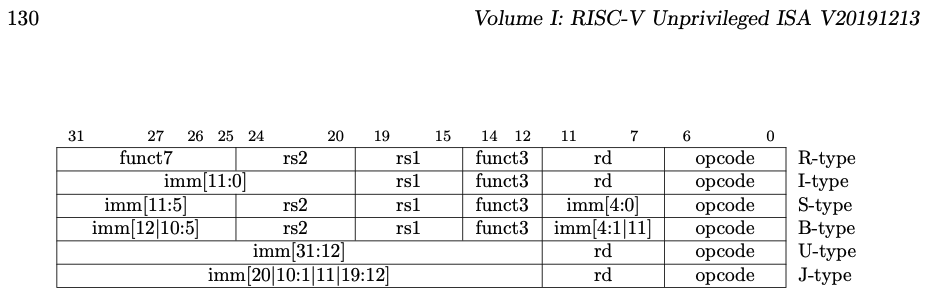
\includegraphics[width=6in,angle=0]{Figures/Fig_Instr_Encodings}}}
  \caption{\label{Fig_Instr_Encodings} RISC-V Instruction Encodings}
\end{figure}
The labels on the right-hand-side are suggestive of the class of
instructions that use that coding:
\begin{tightlist}
  \item R: ``register class'': typically two register inputs
  \item I: ``immediate class'': typically one register and one immediate input
  \item S: ``store class'': for the STORE instructions SB, SH and SW
  \item B: ``branch class'': for the conditional branch instructions
  \item U: ``Upper Immediate class'': for LUI (Load Upper Immediate)
        and AUIPC (Add Upper Immediate to PC)
  \item J: ``Jump class'': for jump instructions JAL and JALR
\end{tightlist}

We use standard Verilog ``bit-slice'' notation to refer to bit-fields
of the 32-bit instruction. Thus, instr[6:0] refers to the lower 7 bits
(bits 0 through 6) of the 32-bit instruction.

The overall ``operation code'' (opcode) of an instruction is a
combination of 6-bit \verb|opcode| field in instr[6:0] and the funct3
and funct7 fields at other positions in the instruction.

If the instruction reads at least one register, the first one is
specified in the rs1 field (``register source 1''); the 5 bits in
instr[15-19] specify one of the 31 registers.  If the instruction
reads two register, the second one is specified in the rs2 field; the
5 bits in instr[24-20] specify one of the 31 registers.  If the
instruction writes a register, it is specified in the rd field
(``register destination''); the 5 bits in instr[11-7] specify one of
the 31 registers.

In RISC-V, reading register \verb|x0| always yields the value 0.  This
is a useful convenience built into the ISA.  For example, there is an
instruction to test if the rs1-value is less than the rs2-value.  If
we specify \verb|x0| for rs2, then we effectively test if the rs1
value is negative.

Some instructions take input data from bits in the instruction itself;
these are called ``immediate'' fields.  In
Figure~\ref{Fig_Instr_Encodings} we can see that there are various
encodings for the immediate fields.  Consider the J-type instruction.
Figure~\ref{Fig_J_imm} shows how the 20 ``imm'' bits in the
instruction are permuted, with a 0 bit appended to the right, to
produce a 21-bit immediate value to be used in the computation.
\begin{figure}[htbp]
  \centerline{
\includegraphics[width=6in,angle=0]{Figures/Fig_J_imm}}
  \caption{\label{Fig_J_imm} Construction of 21-bit immediate from 20 ``imm'' bits in J-type instructions}
\end{figure}

Similarly, Figure~\ref{Fig_B_imm} shows how the 12 ``imm'' bits in the
instruction are permuted, with a 0 bit appended to the right, to
produce a 13-bit immediate value to be used in the computation.
\begin{figure}[htbp]
  \centerline{
\includegraphics[width=6in,angle=0]{Figures/Fig_B_imm}}
  \caption{\label{Fig_B_imm} Construction of 13-bit immediate from 12 ``imm'' bits in B-type instructions}
\end{figure}

In both of the above, the encoding takes advantage of the fact that
Jump and Branch target PCs are always at least 2-byte aligned, and
therefore we do not have to use up an instruction ``imm'' bit to
represent the ``0'' least-significant bit.  The extra bit in the
immediate value effectively doubles the ``distance'' that a jump or
branch can span.\footnote{Actually in RV32I and RV64I PC targets are
4-byte aligned. The 2-byte alignment here accomodates the optional C
(Compressed) extension, where instructions may be only 2-byte
aligned.}

The fact that there are so few encoding formats justifies the ``RISC''
in the ISA name: Reduced Instruction Set Computer.  Having fewer
formats, with few or zero special cases, simplifies the hardware
needed to decode an instruction.

% ****************************************************************

\section{Unprivileged ISA RV32I}

\label{Sec_RV32I}

\index{RISC-V!ISA!RV32I base integer instructions}

Figure~\ref{Fig_RV32I_labeled} reproduces the table on page 130 of the
RISC-V Unprivileged ISA specification, which shows all RV32I
instructions.
\begin{figure}[htbp]
  \centerline{\frame{\includegraphics[width=6in,angle=0]{Figures/Fig_RV32I_labeled}}}
  \caption{\label{Fig_RV32I_labeled} RISC-V RV32I Instructions}
\end{figure}
On the right-side of the diagram we have labeled different classes of
instructions.

Note that there are just 40 instructions (again justifying the ``RISC'' name).

% ================================================================

\subsection{``Upper Immediate'' instructions LUI and AUIPC}

Figure~\ref{Fig_LUI_AUIPC} reproduces the top of page 19 of the RISC-V
Unprivileged ISA specification, which describes the semantics of the
LUI and AUIPC instructions in prose text.
\begin{figure}[htbp]
  \centerline{\frame{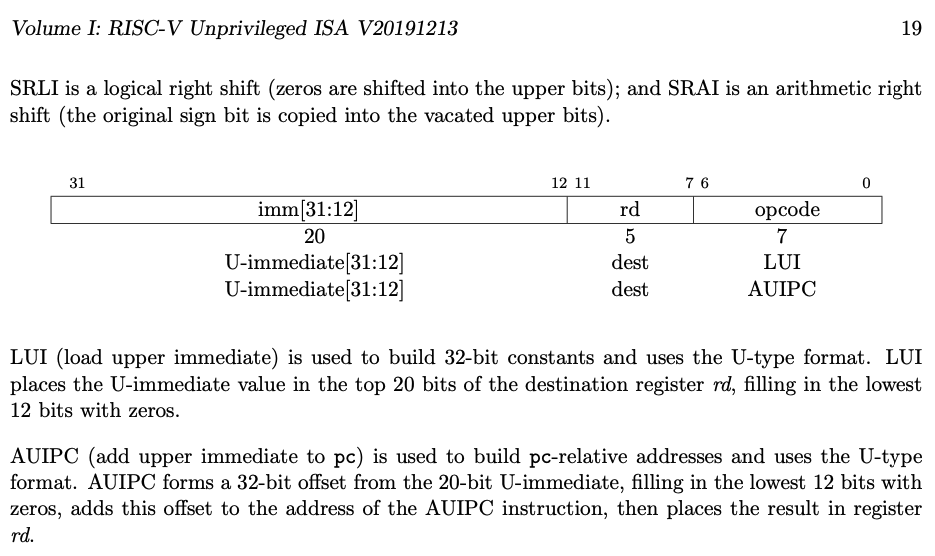
\includegraphics[width=5in,angle=0]{Figures/Fig_LUI_AUIPC}}}
  \caption{\label{Fig_LUI_AUIPC} RISC-V LUI and AUIPC Instruction semantics}
\end{figure}

Figure~\ref{Fig_LUI} is a pictorial depiction of the semantics of an LUI instruction.
\begin{figure}[htbp]
  \centerline{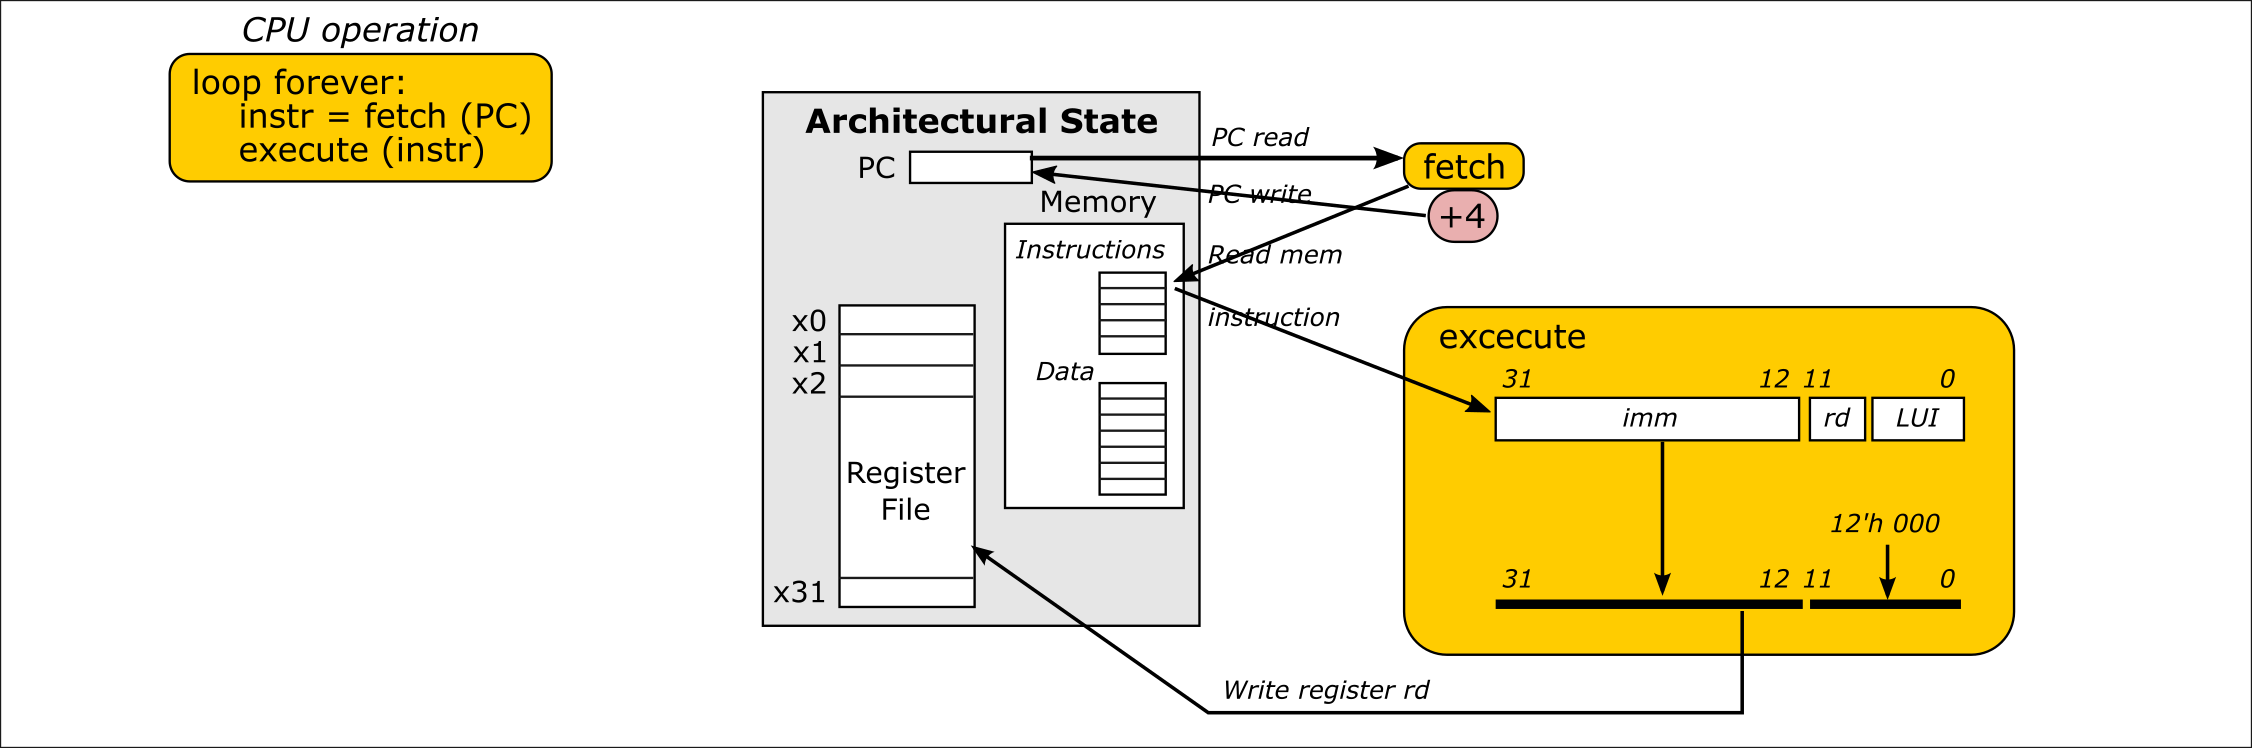
\includegraphics[width=6in,angle=0]{Figures/Fig_LUI}}
  \caption{\label{Fig_LUI} Execution semantics for LUI instructions}
\end{figure}
At the left of the figure is depiction of the general behavior of a
CPU, namely to loop forever, at each iteration fetching the
instruction that is in memory at the address specified by the PC
register, and then executing that instruction.  For the LUI
instruction, to the 20 bits [31:12] of the instruction (the
``immediate'' value) we append twelve bits of constant 0 as
least-significant bits to construct a 32-bit value.  This value is
then written into register rd.

Figure~\ref{Fig_AUIPC} is a pictorial depiction of the semantics of an AUIPC instruction.
\begin{figure}[htbp]
  \centerline{\includegraphics[width=6in,angle=0]{Figures/Fig_AUIPC}}
  \caption{\label{Fig_AUIPC} Execution semantics for AUIPC instructions}
\end{figure}
As with LUI, to the 20 bits [31:12] of the instruction (the
``immediate'' value) we append twelve bits of constant 0 as
least-significant bits to construct a 32-bit value.  For AUIPC we add
this value to the 32-bits of the PC, and the result is then written
into register rd.

% ================================================================

\subsection{Conditional BRANCH instructions}

Conditional branch instructions compare the values in registers rs1
and rs2 for some condition: BEQ (equal), BNE (not-equal), BLT
(less-than), BGE (greater-than-or-equal).  If the condition is:

\begin{tightlist}

  \item false (``branch not taken''):

    \begin{tightlist}
      \item The instruction is a no-op, it just falls through to the
            next instruction (PC := PC+4).
    \end{tightlist}

  \item true (``branch taken''):

    \begin{tightlist}
      \item The 12 ``imm'' bits form a 13-bit value (see
            Figure~\ref{Fig_B_imm}).

      \item This 13-bit value is sign-extended to 32 bits and added to
            the current PC to form a target address (``branch
            target'').
            
      \item The PC is updated to contain the target address.
    \end{tightlist}

\end{tightlist}

Because of sign-extension (+/-), the branch may be forwards or
backwards relative to the current PC.

For BLT and BGE, the comparison treats the two input 32-bit values as
\emph{signed} values.  For BLTU and BGEU, they are treated as
\emph{unsigned} values.

% ================================================================

\subsection{LOAD and STORE memory-access instructions}

LOAD (LB, LH, LW, LBU, LHU) instructions move data from memory into a
register.  STORE (SB, SH, SW) instructions move data from a register
to memory.  In both cases, the address is formed by sign-extending the
12-bit immediate value to 32 bits and adding it to the value from
register rs1.  For LOAD instructions, the value loaded is placed into
register rd.  For STORE instructions, the value in register rs2 is
stored to memory, and there is no result value written into any
register.

As with most modern ISAs, RISC-V memory is byte-addressed, {\ie} each
address refers to a specific byte in memory.  The size of the data to
be loaded/stored is given by ``B'' (1 Byte), ``H'' (Halfword = 2
bytes), or ``W'' (Word = 4 bytes) in the instruction name.

The difference between LB and LBU is whether the 8 bits loaded (1
byte) are sign-extended or zero-extended, respectively, to 32 bits
when placed in the 32-bit rd. (And similarly for LH vs. LHU.)

How to read the ISA spec: examples LOAD/STORE, Register-Register
Arithmetic and Logic, Register-Immediate Arithmetic and Logic,
Unconditional Jump.

% ================================================================

\subsection{Register-Register Arithmetic and Logic instructions}

These instructions read registers rs1 and rs2, perform the specified
arithmetic/logic operation on the two values, and store the result
into register rd.

SLT (``set if less than'') tests if register[rs1] < register[rs2], and
writes 0 (false) or 1 (true) into the destination register, treating
the inputs as 32-bit signed values.  SLTU treats inputs as unsigned
values.

SRL (``shift right logical'') shifts the value from register[rs1] to
the right (towards the least-significant bits) by the amount in
register[rs2].  Zeroes are shifted in from the left.

In SRA (``shift right arithmetic''), the register[rs1][31] is shifted
in from the left, {\ie} the 32-bit value is treated as a signed
integer (bit 31 is the sign bit).

In SLL (``shift left logical''), zeroes are shifted in from the right.

In all three shifts, since there are only 32 bits in register[rs1],
only the lower 5 bits of register[rs2] are relevant ({\ie} bits
[4:0]); the rest are ignored.

% ================================================================

\subsection{Register-Immediate Arithmetic and Logic instructions}

These instructions read register rs1, form a signed 32-bit value from
the 12-bit ``imm'' bits, and perform the specified arithmetic/logic
operation on the two values, and store the result into register rd.

In SRLI (``shift right logical immediate''), SRAI (``shift right
arithmetic immediate''), and SLLI (``shift left logical immediate''),
the 5-bit \verb|shamt| field provides the ``shift amount''.

% ================================================================

\subsection{Unconditional Jump instructions}

JAL (``jump and link'') forms a 21-bit value from the 20 ``imm'' bits
(see Figure~\ref{Fig_J_imm}), sign-extends it to 32 bits, adds it to
the current PC value and updates the PC with the result.

JALR (``jump and link register'') forms a 12-bit value from the 12
``imm'' bits, sign-extends it to 32 bits, adds that to the value in
register[rs1], forces bit [0] to be 0, and updates the PC to that
value

Both JAL and JALR store the current PC + 4 (``return address'') into
register[rd].

These are most often used for subroutine calls and returns.
Figure\ref{Fig_JAL_JALR} illustrates the protocol.
\begin{figure}[htbp]
  \centerline{\includegraphics[width=6in,angle=0]{Figures/Fig_JAL_JALR}}
  \caption{\label{Fig_JAL_JALR} JAL and JALR for subroutine call and return}
\end{figure}

Suppose, inside function f1(), at address x, we have a {\tt JAL ra,f2}
instruction representing a subroutine call to function f2().  The
compiler/linker will place ``delta'' in the JAL instruction's
``immediate'' field, where delta is the difference between x and the
entry point of f2().  In RISC-V Assembly Language, ``ra'' (``return
address'') is another name for register[1], which is used to hold
return addresses as part of the standard software calling convention.
The JAL instruction saves x+4 (the return address) in register ra, and
sets the PC to x+delta, so that the next instruction fetched will be
the entry point of f2().

Inside f2(), at address y, suppose we have a {\tt JALR 0,ra,0}
instruction representing the return to the caller.  It saves y+4 in
register 0, but recall that writes to register 0 are always ignored.
It reads the value in register ra, adds 0 to it and sets the PC to the
result value, {\ie} the next instruction fetched will be from x+4.

JAL is used for most subroutine calls which are to a manifestly known
subroutines (so the compiler/linker can compute the ``delta'' for the
immediate value).  JALR is used for subroutine calls where the
``delta'' is not known to the compiler/linker, for example when
calling through a table of function pointers.

JALR is also used for subroutine calls and returns and conditional
branches to ``distant'' target addresses.  Remember that BRANCH
instructions only have a 13-bit signed offset from the current PC, and
JAL only has a 21-bit signed offset.  For more distant jumps, we can
construct a full 32-bit value in a register (using one or more LUI and
AUIPC instructions, for example) and then use that as the jump rs1 in
a JALR instruction.

% ****************************************************************

\section{Traps due to illegal instructions and other exceptions}

\label{Sec_Traps}

Most processors cannot afford to get ``stuck'' on an unrecognized
instruction (illegal instruction).  An illegal instruction raises one
of several possible ``exceptions''.  Other events that raise
exceptions are misaligned memory access (in FETCH or LOAD/STORE), or a
memory-access to an unimplemented address (in FETCH or LOAD/STORE),
{\etc}.

% ----------------
\vspace{2ex}

NOTE:
\fbox{\small
\begin{minipage}{5in}

``Illegal'' just means: outside the currently implemented subset. For
example (see Figure~\ref{Fig_ISA_Modularity}), a legal RISC-V
instruction in, say, the M extension is considered illegal in an
implementation that only implements the RV32I subset.

\end{minipage}}

\vspace{2ex}
% ----------------

Exceptions are treated like an ``unexpected call'' to a special
subroutine called a ``trap handler''.  The architectural state is
extended with a few extra registers belonging to a class of registers
called CSRs (Control and Status Registers), shown in
Figure~\ref{Fig_Trap_CSRs}.
\begin{figure}[htbp]
  \centerline{\includegraphics[width=6in,angle=0]{Figures/Fig_Trap_CSRs}}
  \caption{\label{Fig_Trap_CSRs} CSRs for handling traps}
\end{figure}

To ``return'' from a trap handler we need one more instruction: MRET,
which is in the ``RISC-V Privilege M ISA'' (see
Figure~\ref{Fig_ISA_Modularity}).  Figure~\ref{Fig_Trap_Return}
illustrates the flow into the trap handler and back on an exception
(an ILLEGAL instruction is one possible cause of the exception).
\begin{figure}[htbp]
  \centerline{\includegraphics[width=6in,angle=0]{Figures/Fig_Trap_Return}}
  \caption{\label{Fig_Trap_Return} Trap and return flow}
\end{figure}

When the exception is detected, the hardware saves the faulting PC
(PCx in the figure) in CSR MEPC, saves a cause-code in CSR MCAUSE and
possibly one more piece of data (depending on the type of exception)
in CSR MTVAL.  Then, it sets the PC to the value in MTVEC, so that we
start executing the trap-handler code.

When the trap-hanlder has finished, it executes an MRET instruction
which copies the value in MEPC into the PC, continuing execution at
that location.

Exception-cause codes relevant to this book (RV32I + exception
handling) are shown in the table below (excerpted from Table 3.6 in
the Privileged ISA Specfication document).

\begin{center}
 \begin{tabular}{|c|l|}
  \hline
  Exception-Cause code & Description \\
  \hline
  0 & Instruction address misaligned \\
  1 & Instruction access fault \\
  2 & Illegal instruction \\
  3 & Breakpoint \\
  4 & Load address misaligned \\
  5 & Load access fault \\
  6 & Store/AMO address misaligned \\
  7 & Store/AMO access fault \\
  ... & ... \\
  11 & Environment call M-mode \\
  ... & ... \\
  \hline
 \end{tabular}
\end{center}

The trap handler code can examine MCAUSE, MEPC and MTVAL to determine
what it should do to handle the trap.  Regarding MEPC, it may:
\begin{itemize}

 \item Leave MEPC untouched, so that, on MRET, we retry the
       exceptional instruction.

       \emph{Example}: the exception was a page-fault due to a FETCH
       on an umapped page.  The trap handler may map the page, and
       MRET to the faulting instruction to be retried (which,
       hopefully, should not page-fault again).

 \item Increment MEPC by 4, so that, on MRET, we resume at the next
       instruction after the faulting instruction.

       \emph{Example}: the faulting instruction is a legal RISC-V
       instruction, but has deliberatly been left unimplemented ({\eg}
       to save hardware cost).  The trap handler ``emulates'' the
       instruction ({\ie} performs the required computation using
       implemented instructions), and resumes the normal flow at the
       next instruction.

       \emph{Example}: the trap handler just records that this
       instruction is illegal so that it can avoid it in subsequent
       execution.

 \item Change it to something else entirely, to abandon the current
        ``normal'' flow and do something else.

       \emph{Example}: in an Operating System, we save MEPC for future
       resumption, and change it to give another process a chance to
       execute.
\end{itemize}

% ================================================================

\subsection{ECALL and EBREAK instructions, and Interrupts}

RV32I instructions ECALL and EBREAK are handled just like other
exceptions; in that sense, these are not ``unexpected'' conditions,
but exceptions deliberately induced by the program.  The only notable
feature is that they place certain exception-cause codes in the MCAUSE
CSR (see ``Environment call M-mode'' and ``Breakpoint'', respectively,
in the table above).

In systems with operating systems, ECALL is used to move in a
disciplined way from lower to higher privilege levels (from User mode
to Supervisor mode, and from Supervisor Mode to Machine mode).

Some RISC-V implementations contain a hardware ``Debug Module'', in
which case EBREAK is treated differently (please see the RISC-V Debug
Module specification document).  It is used as part of the
implementation of the ``break'' command in debuggers like GDB, LLDB
and OpenOCD.

An external interrupt is also dispatched into the trap-handler just
like exceptions, the only difference being the code placed in the
MCAUSE register (see Table 3.6 in the Privileged ISA Specfication
document for all the defined interrupt cause codes).

% ================================================================

\subsection{CSRRxx instructions}

In Section~\ref{Sec_Traps} we described how various CSRs are read and
written during trap-handling.  These reads and writes are performed
\emph{by the hardware} as part of taking a trap or performing an MRET.

But we also need a way to read and write CSRs \emph{programmatically},
{\ie} from instructions in the program.  For example, before any trap
is taken, some early part of the execution needs to write the
trap-vector's PC into MTVEC.  During trap-handling, the trap-handler
needs to read (and possibly write) MEPC, MCAUSE and MTVAL.

Programmatic access to CSRs is provided by a family of six ``CSRRxx''
instructions.  The following table is excerpted from the RISC-V
Unprivileged ISA spec document (Chapter 9, on the ``Zicsr''
extension).
\begin{figure}[htbp]
  \centerline{\frame{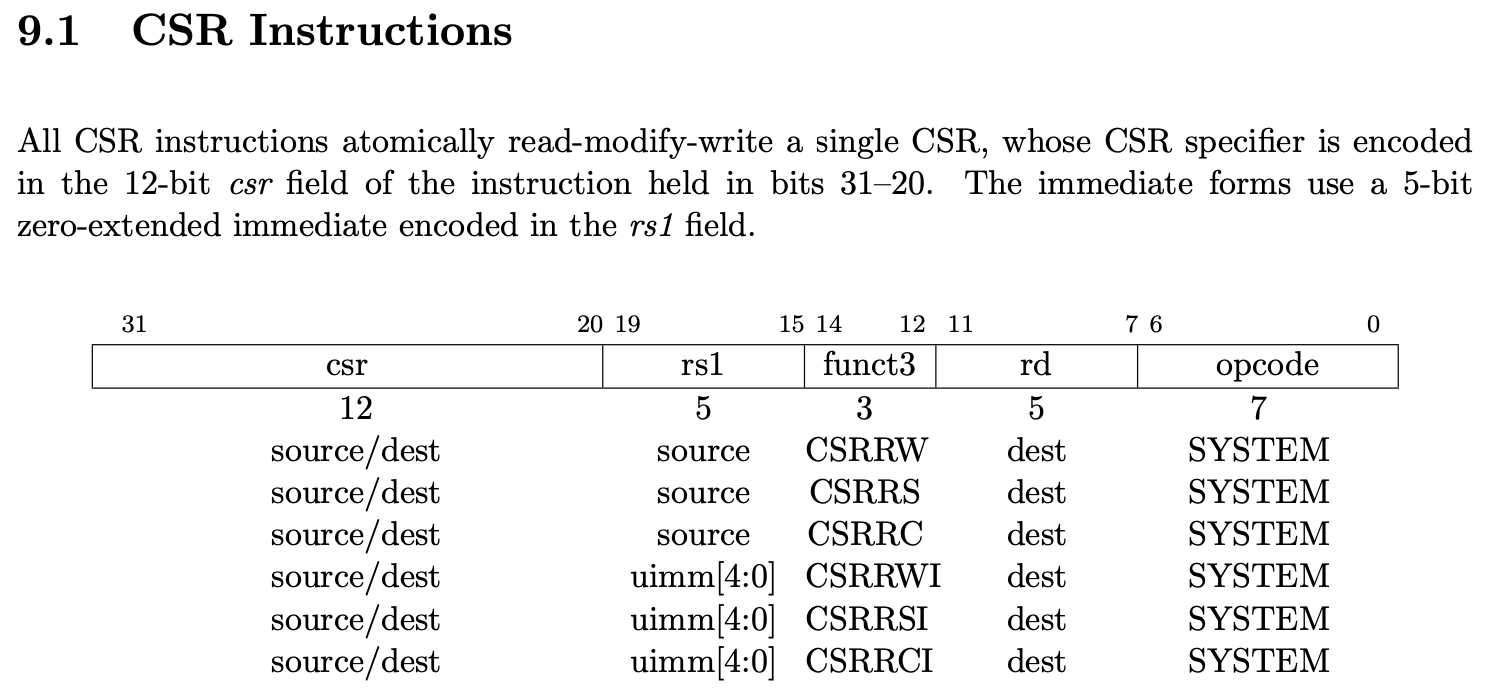
\includegraphics[width=6in,angle=0]{Figures/Fig_CSRRxx_spec}}}
  \caption{\label{Fig_CSRRxx_spec} CSRRxx instructions (from Unprivileged Spec)}
\end{figure}

As the text says, each CSR instruction:

\begin{tightlist}

 \item reads a value $x$ from a general-purpose register (rs1) or
       takes the rs1 field itself as a literal 5-bit value;

 \item reads a value $y$ from a CSR (whose 12-bit address is given in
       \verb|instr[31:20]|);

 \item returns $y$ into a general-purpose register (rd);

 \item and writes back a value into the CSR that is some function of
       $x$ and $y$ (the details vary across the six CSRRxx
       instructions).

\end{tightlist}
For details, please read the RISV-V Unprivileged ISA specification
document, Chapter 9.


% ================================================================

\subsection{FENCE}

The FENCE instruction is intended for RISC-V implementations that
contain caches in the memory system.  In such systems, data may not
reach memory quickly or at all (is in the cache and is not evicted),
and two items of data $x_1$ and $x_2$ may reach memory in a different
order from the STORE instructions that wrote them (because the order
in which their cache lines are written back to memory has no relation
ship to the program STORE order).

The FENCE instruction is often used to ``push'' data from the cache to
memory, although technically the FENCE instruction only guarantees an
``ordering'', {\ie} that if there are two STOREs $x_1$ and $x_2$
before and after a FENCE, respectively, then $x_1$ will be visible
before $x_2$ to any other agent in the system (another CPU, a DMA
engine, an I/O device, {\etc}).

% ================================================================

\subsection{RV64I differences from RV32I}

The Architectural State for RV64I is just like that for RV32I, except
that the PC and 32 registers are now 64-bits wide instead of 32-bits
wide.  Figure~\ref{Fig_RV64I} reproduces the table of RV64I
instructions from page 131 of the Unprivileged Spec document.
\begin{figure}[htbp]
  \centerline{\frame{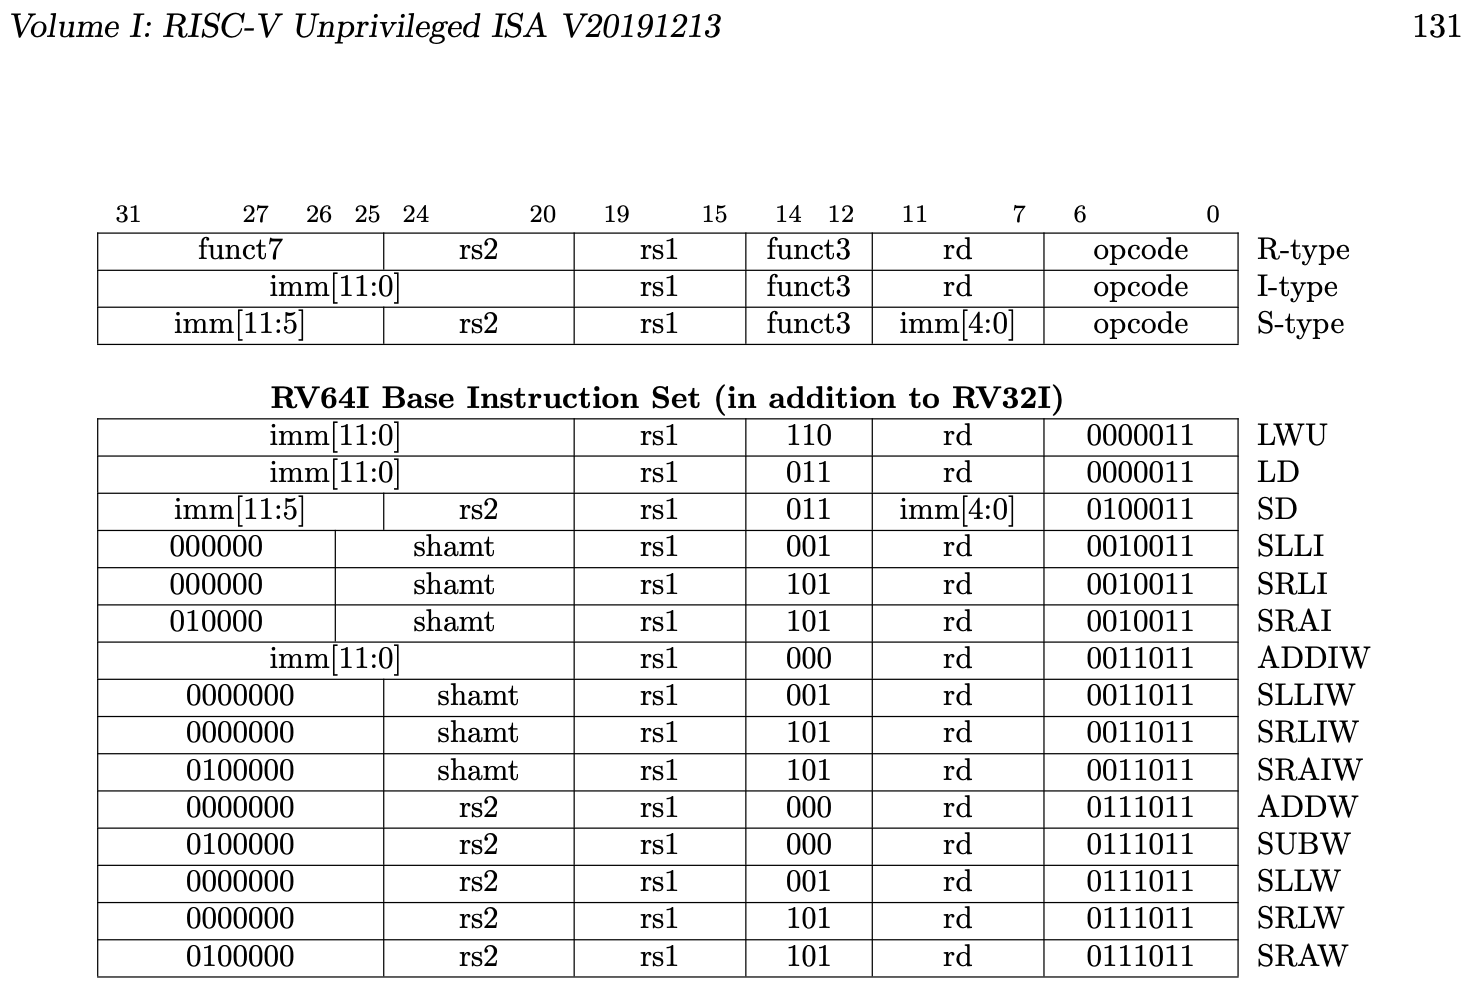
\includegraphics[width=6in,angle=0]{Figures/Fig_RV64I}}}
  \caption{\label{Fig_RV64I} RV64I instructions (in addition to RV32I)}
\end{figure}
RV64I starts with the same forty instructions as in RV32I, except that
it replaces 3 of them---SLLI, SRLI and SRAI---with slight
modifications: the ``shamt'' field is now 6 bits instead of 5, to
accommodate 64-bit shifts.

In RV64I, the LW instruction loads 32-bits from memory, sign-extends
it to 64 bits and stores it in the destination register.  RV64I adds
the LWU instruction that does the same, except that it zero-extends
the 32-bit value from memory.  RV64I also adds the LD instruction to
load 64-bits from memory into a register.

RV64I adds the SD instruction to store a 64-bit value from a register
into memory.

In RV64I, ADDI, SLLI, SRLI, SRAI, ADD, SUB, SLL, SRL and SRA all
operate on 64-bit values.  RV64I adds ADDIW, SLLIW, SRLIW, SRAIW,
ADDW, SUBW, SLLW, SRLW and SRAW to operate on the lower 32-bits of
64-bit register values.

% ****************************************************************

\section{Continued Evolution of the RISC-V ISA (with your contribution?)}

\index{RISC-V!ISA!Evolution of}
\index{RISC-V!ISA!Extensions to}

The RISC-V ISA is not frozen.  As shown in
Figure~\ref{Fig_ISA_Modularity}, the ISA has consciously been designed
in a modular way and to be modularly extensible.  RISC-V International
(RVI, \url{https://riscv.org}) runs an organized process for the
continued maintenance and evolution of the ISA.  Special-interest
groups drawn widely from RVI membership constitute various committees
under the aegis of RVI to propose, develop, and specify new extensions
to the ISA (for cryptography, for image and video manipulation, for
high-performance computing, for AI, and so on).  There is a formal
public-review and ratification process for any new proposed
extensions.

RVI has the usual corporate membership tiers seen in many consortiums
but, unusually, it also has inexpensive memberships for individuals
(students, hobbyists, ...)  and academic institutions.  So please feel
free to join, in order to monitor the RISC-V ecosystem closely or,
even better, to actively contribute to its future,

% ****************************************************************
